\chapter{Determination of the relevant scales}

In this project we base our analysis on the center of galaxy clusters at low redshift so it is necessary to understand which scales will be relevant for our studies. In order to calculate the range of scales that we will probe in the observational procedures on Chapter 4 we will do three separate experiments. 

The first experiment is the calculation of the number of objects that we would expect to be lensed near the cluster centres by using a very extensive catalogue of galaxies located at different redshifts. Calculating the ammount of galaxies that we should see in the vicinity of the BCG (with their reported redshift) given the characteristics of our data gives us an idea on how many of those objects could in principle be lensed by the BCG and what is the redshift range on which me should focus our attention. 

The second experiment consists on doing the mass modelling of the cluster for its stellar and dark matter content to see on which scale stars are the main component of the enclosed mass that lenses background objects (this will suggest where the determination and characterisation of the IMF can be done with a good degree of confidence). 

The third one is the calculation of the expected Einstein radius for objects located at differents redshifts which will help us define the most relevant regions to look for lensing candidates.

\section{Experiment one: COSMOS field}

For our first experiment we need a very large catalogue of galaxies that contains their spatial locations and redshifts because this alows us get the average number of galaxies contained inside a square region (similar to the effective area surrounding the BCGs of our sample) with their corresponding redshifts. This will thus give us the number of galaxies that we would expect to see with the sensitivity of our data and will also help us constrain the redshifts to probe. For this purpose we make use the COSMOS2015 catalogue (\textcolor{blue}{Laigle et al.} \citeyear{Reference21}) which contains half a million objects in a range of $1<z<6$. 

Ricardo Herbonnet (private communication) matched the CFHT data to this catalogue so we use his matched data which contains a total of 133,348 galaxies in the 2 degree COSMOS field. We count the amount of galaxies for different magnitudes in redshift bins of 0.2 $z$ for the $r$ filter. These numbers represent the expected number of galaxies in the background of the lens objects of our sample as seen in Figure [3.1]. 

\begin{figure}[H]
\centering
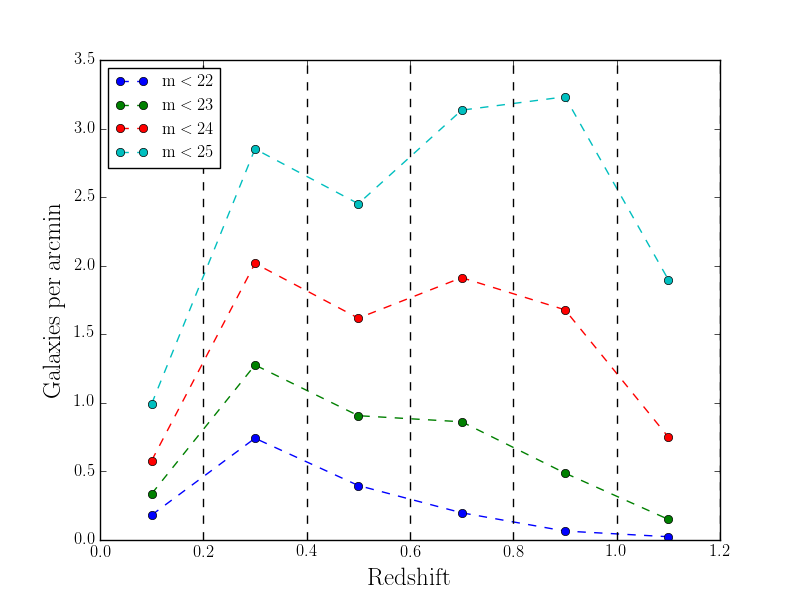
\includegraphics[width=12cm]{images/galaxies_per_arcmin.png}
\caption[Galaxies per arcmin]{Galaxies per arcmin$^2$ in redshift bins of $0.2z$ for different magnitudes. HST could be able to see objetcs with magnitudes below 25 while CFHT can see objects with magnitudes around 23.}
\end{figure}

Around $z=0.3$ we find the peak for the number of galaxies so it is the redshift that is most likely to contain galaxies that could be seen in our data. For the depth of our data of around 23 mag (as discussed in the next chapter) we then expect some background galaxies lensed by the BCGs and for which we can measure the Einstein ring, although the number is rather small. 

CFHT can see objects as deep as $m=23$ but Hubble Space Telescope could see objects with $m=25$ so it should be able to see a lot more objects that have been lensed. This result is a first suggestion that within the inner region of the galaxy clusters, there must be lensed objects in the form of arcs or multiple images that we could be able to see with our sample making a careful subtraction of the BCG light. Now we must answer the question regarding the scales in which the stellar content (associated to the extracted light from the BCG) is relevant.

\section{Experiment two: DM to stellar ratio}

We first need to take into consideration is the density profile that we will use for our calculation of the fraction of DM and stellar light. The first usual approach for the density profile of the gravitational lens is an isothermal sphere (see Appendix), although in reality, the density profile and lensing properties of galaxies is a bit more complicated than the assumption of a SIS (singular isothermal sphere), so we need to take into account more complex but elaborate profiles such as the NFW (\textcolor{blue}{Navarro, Frenk \& White} \citeyear{Reference17}) which is an approximation to the equilibrium configuration of dark matter produced in N-body simulations of colissionless dark matter particles (see Appendix for the formalism of the NFW and it's lensing equations).

So for our second experiment proposed at the beginning of the chapter, we will use the galaxy cluster Abell 1068, located at a distance of $z=0.138$ with magnitudes in $U=21.94$, $i=18.46$, $g=20.09$, $r=19.5$, also $\text{M}_{200}=4.3\times 10^{14}$ $\text{M}_{\odot}$ (\textcolor{blue}{Van der Burg et al.} \citeyear{Reference2}) and calculate its NFW dark matter halo profile (since galaxy clusters are known to be dominated by their dark matter content) and at the same time we calculate its stellar mass profile using the de Vaucouleurs surface brightness profile by \textcolor{blue}{de Vaucouleurs} (\citeyear{Reference32}) which is a specific case of a Sersic's more general profile. This allows us to compare the contribution of stars in comparison to dark matter and thus see in which scales the DM mass becomes dominant thus making it more difficult to constrain the stellar content of the bright galaxy.

The concentration parameter for the NFW profile of this cluster is $c=4.46$ (using Figure [1] in the Appendix). The critical density is 212 $\text{M}_{\odot}/\text{kpc}^{3}$. The Hubble parameter at $z=0.138$ is $H(z)=85.6$. For an effective radius of $R_{e}=73.7$ kpc we get a characteristic radius of $r_{1/2}=307.1$ kpc.

For the stellar content of the cluster we can use de Vaucouleurs law for the surface brightness distribution in giant elliptical galaxies which is:

\begin{equation}
I(R)=I_{e}e^{-b\left[\left(R/R_{e}\right)^{1/4}-1\right]}
\end{equation}

where $b=7.67$ and $I_{e}$ is the effective brightness which is basically the brightness at the effective radius $R_{e}$

For constant mass-to-light-ratio we have $\Sigma_{\star}(R)= \Upsilon I(R)$ (\textcolor{blue}{Lokas \& Mamon} \citeyear{Reference14}) where  $I(R)\approx 10^{7}$ $\text{M}_{\odot}/\text{kpc}^{2}$ was found by fitting the surface brightness with \texttt{GALFIT} (as will be discussed in the next chapter). The mass to light ratio for a Salpeter IMF is $\Upsilon\approx 4$ so the stellar mass profile can be easily calculated with  $\Sigma_{\star}(R)= 4I(R)$. The bolometric luminosity of Abell 1068 is $10^{44}$ erg/s that in solar luminosities is $1.9\times 10^{12}$ $L_{\odot}$, this gives an effective brightness of $0.962\times 10^{7}$ $\text{M}_{\odot}/\text{kpc}^2$. 

Hence we have the surface mass density for both the stellar content and the NFW profile, as shown in Figure [3.2].

\begin{figure}[H]
\centering
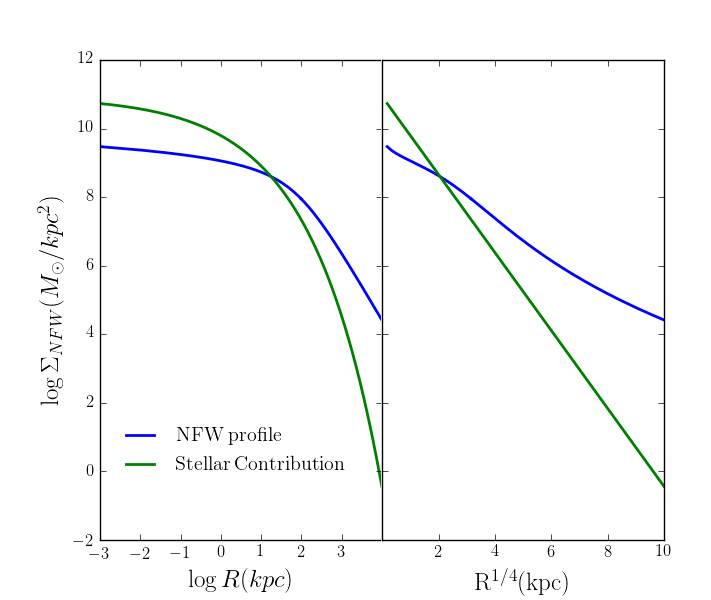
\includegraphics[width=12cm]{images/Surface_mass_density_log.png}
\caption[Surface mass density profiles]{Surface mass density profiles in logarithmic and $R^{1/4}$ scale for the NFW profile and the stellar component.}
\end{figure}

But we are interested in the enclosed mass which can be found by integrating the surface densities. For the DM halo:

\begin{equation}
\textrm{M}(R)=2\pi \int_{0}^{R} R\Sigma(R)dR
\end{equation}

We can recover the luminosity by integrating the surface brightness profile accordingly:

\begin{equation}
L=2\pi \int_{0}^{R} RI(R)dR
\end{equation}

Let's introduce the dependence on different IMFs, mainly Salpeter, Chabrier and Kroupa. Salpeter initial mass function is of the form $n(\textrm{M})\propto \textrm{M}^{-2.3}$ and implies that more low-mass stars and a higher mass-to-light ratio so for massive galaxies  Salpeter is a good IMF. 

In the R-band the scaling between the three IMFs is $\Upsilon_{\text{Krou}}\approx 0.67$ $\Upsilon_{\text{Salp}}$ for Kroupa and $\Upsilon_{\text{Chabrier}}\approx 0.63$ $\Upsilon_{\text{Salp}}$ for Chabrier. The systematic variation of the IMF in early-type galaxies can be seen in Figure [2] from the Appendix. The integration for these different IMFs give a value that is comparable to the one found using Faber-Jackson relation which is $L=\Upsilon\times\sigma^{4}$. 

\begin{center}
\begin{tabular}{c c}
IMF/Method & Mass ($\text{M}_{\odot}$)\tabularnewline
\hline 
\hline
Salpeter & $4.82\times10^{12}$\tabularnewline
Kroupa & $3.13\times10^{12}$\tabularnewline
Chabrier & $3.03\times10^{12}$\tabularnewline
Faber-Jackson & $2.2\times10^{12}$\tabularnewline
DM Halo & $4.63\times10^{14}$\tabularnewline
\end{tabular}
\end{center}

The value found for the enclosed mass for the NFW profile is similar to the one found by \textcolor{blue}{Sifon et al.} (\citeyear{Reference9}) of $4.3\times 10^{14}$ $\text{M}_{\odot}$.

Now let's analyse the radial profiles of these enclosed masses since it is the plot that shows what radial scale we need to probe. We calculate this profiles using equations [5], [7], and [9] from the NFW profile formalism included in the Appendix. The enclosed mass profile for dark matter and stellar matter for the three chosen IMFs (Chabrier, Kroupa, Salpeter) is shown in Figure [3.3].

\begin{figure}[H]
\centering
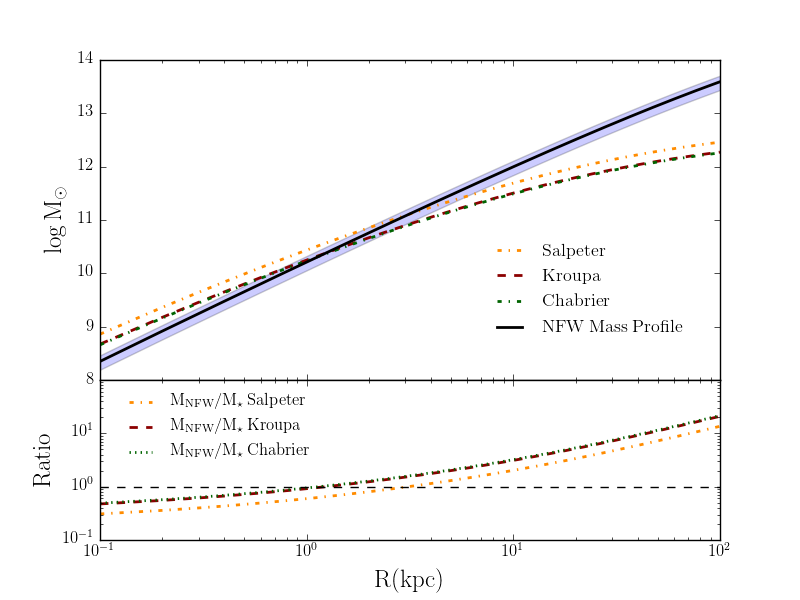
\includegraphics[width=12cm]{images/DM_fraction_all_IMFs.png}
\caption[Enclosed mass and DM to stellar mass ratio for a galaxy cluster]{Top panel: Enclosed mass in DM and stellar content for the chosen IMFs for the galaxy cluster ABELL1068. Bottom panel: DM to stellar mass ratio. Note that the two contributions overlap around $1.5 $ kpc, that is, the very inner region of the galaxy cluster.}
\end{figure}

This result suggests that it is very difficult to make a detailed study if the stellar content of the BCG because the gravitational lensing associated to it would be mostly caused by the dark matter component at almost all scales. The stellar content is only dominant in the innermost region, quite far from the Einstein radius which is constrained by the total enclosed mass (dark matter and stars).

It is then useful to study cases in which the lens system is an elliptical galaxy following its own dark matter halo and not inside the potential well of a galaxy cluster in the case of the BCG. If we now do the calculations for a galaxy with a characteristic radius of $r_s=25.2$ kpc and concentration parameter $c=7.94$ we get:

\begin{center}
\begin{tabular}{c c}
IMF/Method & Mass ($\text{M}_{\odot}$)\tabularnewline
\hline 
\hline
Salpeter & $2.62\times10^{11}$\tabularnewline
Kroupa & $1.70\times10^{11}$\tabularnewline
Chabrier & $1.6\times10^{11}$\tabularnewline
DM Halo & $3.3\times10^{12}$\tabularnewline
\end{tabular}
\end{center}

And the radial profiles in the case of the galaxy are shown in Figure [3.4], where the overlapping happens in a larger radius.

\begin{figure}[H]
\centering
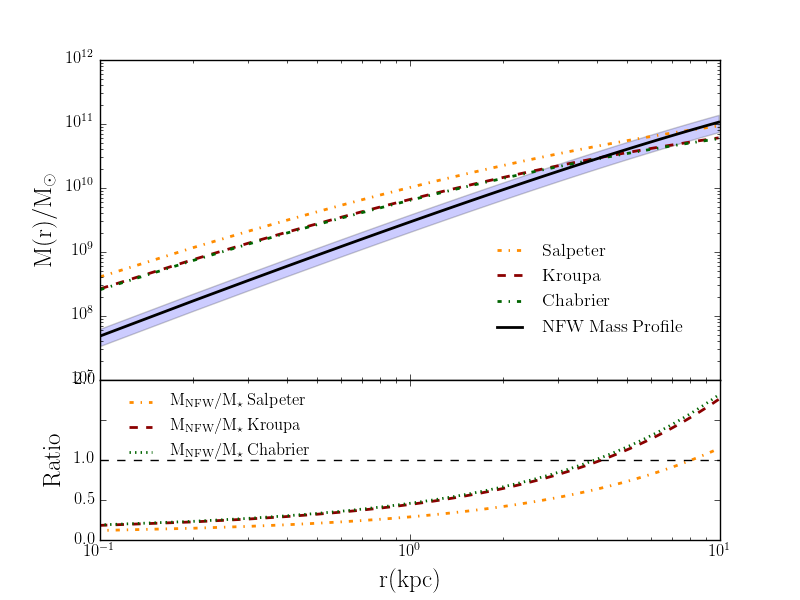
\includegraphics[width=12cm]{images/DM_fraction_all_IMFs_galaxy.png}
\caption[DM and Stellar mass profiles for a massive early type galaxy.]{Top panel: Enclosed mass in DM and stellar content for the chosen IMFs for an early type galaxy. Bottom panel: DM to stellar mass ratio. The two contributions overlap around 3 kpc, further from the center than in the case of the galaxy cluster.}
\end{figure}

Our result is in good concordance with the alalysis made by \textcolor{blue}{Sonnenfeld et al.} (\citeyear{Reference15}) in the system SDSSJ0946+1006, also known as the ``Jackpot". The overlapping of both contributions is around is $~3$ kpc which is a larger radius than the one calculated for a BCG, (see Figure [3.5] for his results). The values for Sonenenfield's galaxy are $z=0.222$, $c=10^{0.9}=7.9428$, $\delta_c=25644.5$, $\text{M}_{\star}=5.5\times 10^{11}$ $\text{M}_{\odot}$.

\begin{figure}[H]
\centering
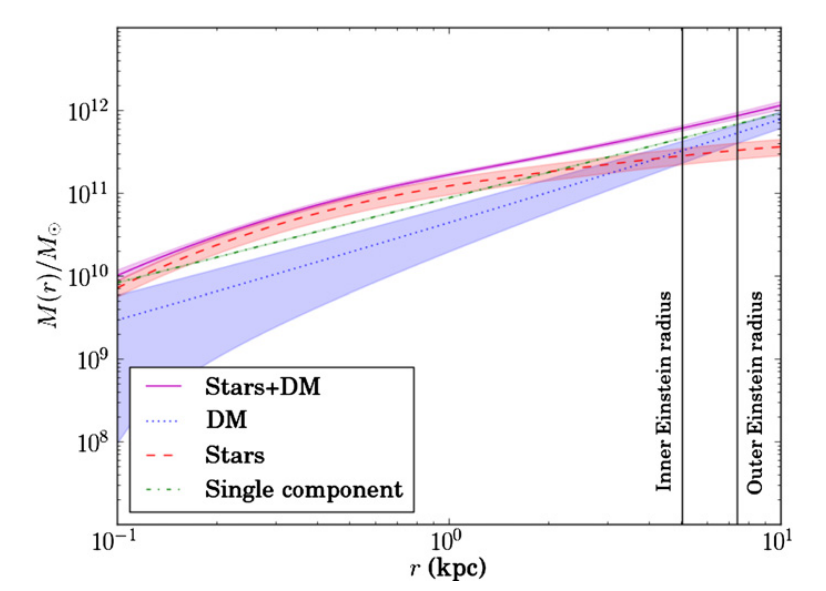
\includegraphics[width=12cm]{images/sonnenfeld_galaxy.png}
\caption[DM and Stellar mass profiles for the ``Jackspot" galaxy.]{Mass profile for dark matter and stellar content for the lens system SDSSJ0946+1006  by \textcolor{blue}{Sonnenfeld et al.} (\citeyear{Reference15}). The overlapping of DM and stellar content is in good agreement with our calculations.}
\end{figure}

This first results mean that the proper determination of the light of the BCG (and thus tracking their formation history through an accurate determination of their IMFs) is harder to do in the inner region of galaxy clusters than it is in early type galaxies in different spatial locations. Dark matter seems to be the overwhelming dominant contribution in the bright galaxies even in the inner regions.

\section{Experiment three: Einstein Radius}

Our third experiment is another way to constrain the relevant scales in which we might expect to see lensed objects. This is done by using the lensing equations to find the Einstein radius in every case (for theoretical background objects located at different redshifts). Calculating the location of the Einstein rings is important because it is around their radial distance from the center of the BCGs that we expect to find arcs or multiple images of background objects, as displayed in Figure [3.6]. 

\begin{figure}[H]
\centering
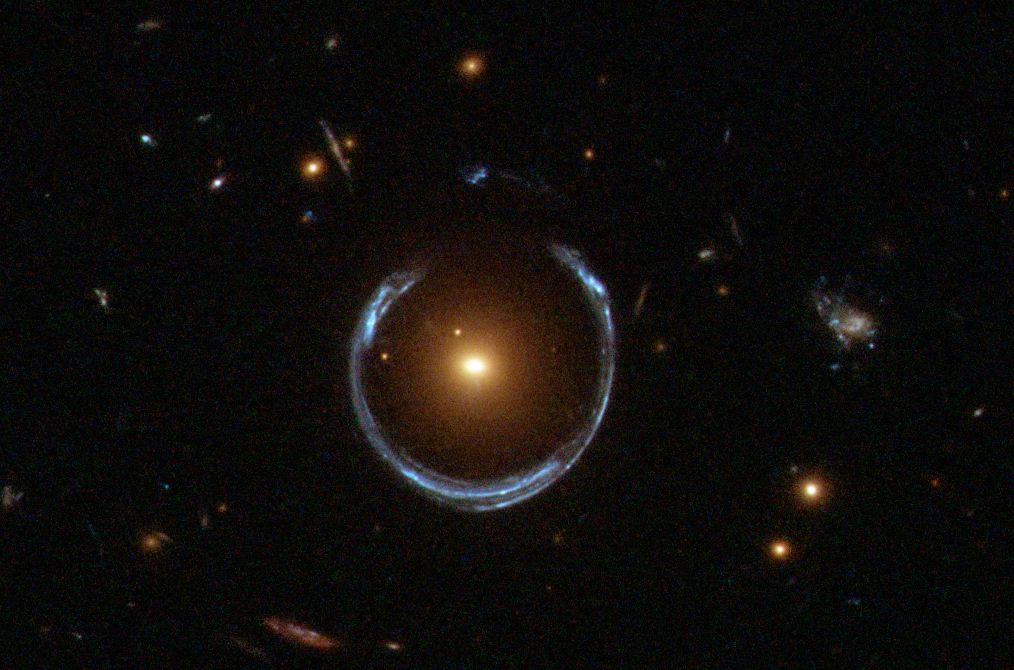
\includegraphics[width=12cm]{images/einstein_ring_wiki.jpg}
\caption[Einstein Ring in LRG 3-757]{Einstein Ring in LRG 3-757 obtained by the Hubble Space Telescope. The distortion produced by the foreground galaxy ($z=0.4457$) is such that the light of the background galaxy ($z=2.379$) is stretched along the Einstein radius as well as being magnified. Image from Wikipedia.}
\end{figure}

Since we are interested in having an accurate estimate of the Einstein radius for objects whose redshift is unknown to us, we use a range of redshifts  $0.1<z<1$ and use the NFW density profile (see Appendix) to compute some quantities that would lead us to the radial distances of the Eintein rings such as the reduced shear and magnification (introduced in Chapter 2). Again, we display the results for the cluster Abell 1068.

The reduced shear for background objects at different redshifts is shown in Figure [3.7] as computed by equation [2.18] and equations [7] and [10] from the Appendix. The radius in which the reduced shear diverges is where the Einstein radius would be located for each of the background objects at the different given redshifts. 

\begin{figure}[H]
\centering
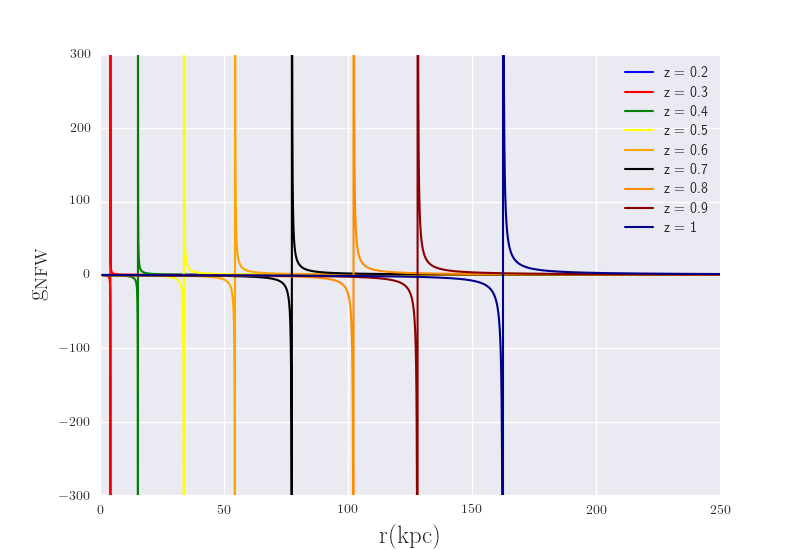
\includegraphics[width=12cm]{images/Reduced_Shear.png}
\caption[Reduced shear radial]{Reduced shear radial profile for different redshifts for Abell 1068. The divergence occurs in the location of the Einstein ring.}
\end{figure}

Another useful way to constrain the Einstein radius is through the magnification given by equation [2.19] and equations [7] and [10] from the Appendix.
 
Figure [3.8] shows the magnification. The infinite magnification happens in the Einstein radius so this is also a useful plot for the radial scales in which we might expect to find lensed galaxies.

\begin{figure}[H]
\centering
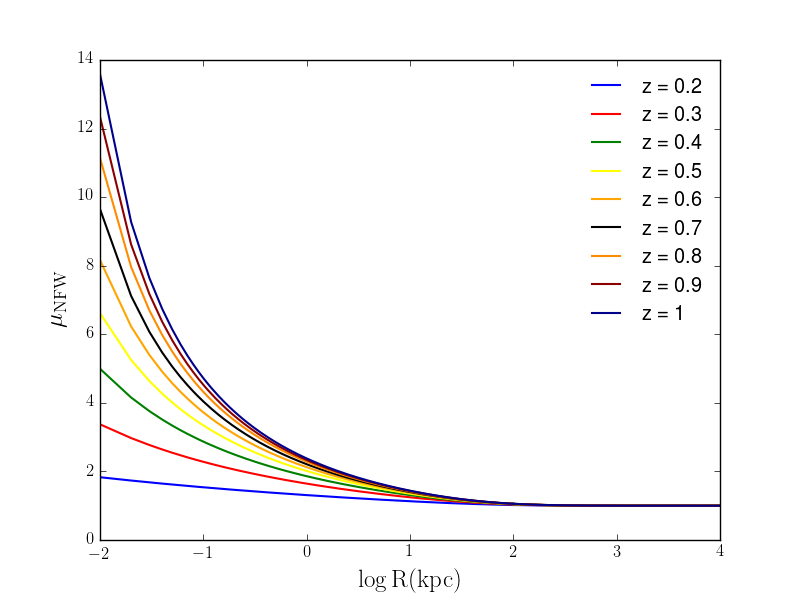
\includegraphics[width=12cm]{images/Magnification.png}
\caption[Magnification radial profile]{Magnification radial profile for various redshifts for Abell 1068. Divergence occurs in the location of the Einstein ring.}
\end{figure}

Taking into account the COSMOS catalogue experiment, and the plots for the reduced shear and the magnification, we would expect to find at least 1 or 2 lensed galaxies near a radial distance from the center of about $15$ kpc, although we know that the enclosed mass at this range is already mostly dominated by the DM halo. 

\begin{comment}
Finally, the shear dependence on radius is shown in Figure [3.10] (See Appendix).

\begin{figure}[H]
\centering
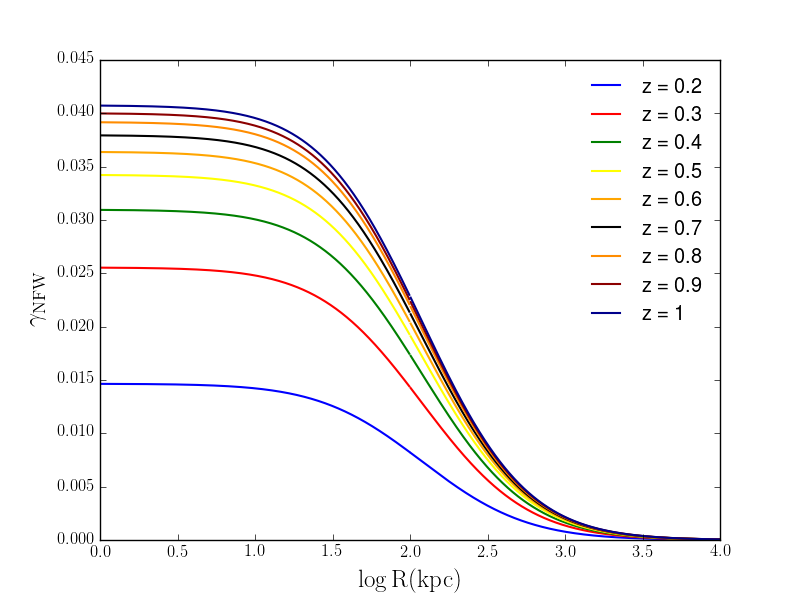
\includegraphics[width=12cm]{images/Shear_vs_rad.png}
\caption[Shear dependence on radius]{Shear dependence on radius for different redshift of the background galaxies}
\end{figure}
\end{comment}